\documentclass[crop,tikz]{standalone}

\usepackage[utf8]{inputenc}

% 'crop' is the default for v1.0, before it was 'preview'
%\usetikzlibrary{...}% tikz package already loaded by 'tikz' option
\usetikzlibrary{arrows} 

\newcommand{\cross}[2]{
	\draw[fill=black!20!white] (-#2,-#1) -- (-#1,-#1) -- (-#1,-#2) -- (#1,-#2) -- (#1,-#1) -- (#2,-#1) -- (#2,#1) -- (#1,#1) -- (#1,#2) -- (-#1,#2) -- (-#1,#1) -- (-#2,#1) -- cycle;
} %\cross{thickness/2}{arm length/2}

\begin{document}

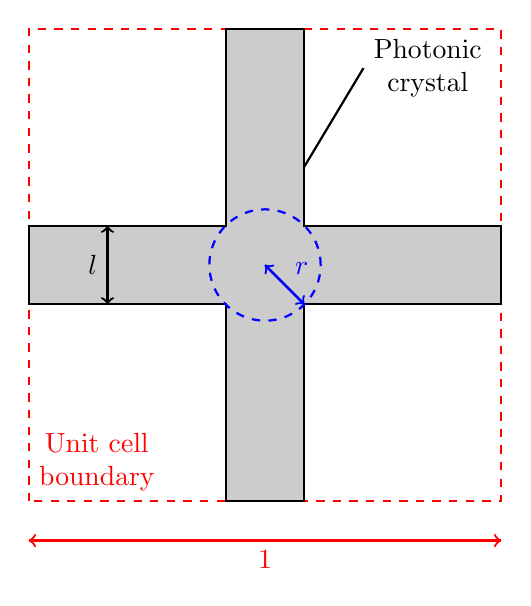
\begin{tikzpicture}[thick, main node/.style={circle,draw,font=\sffamily\Large\bfseries}]
	%periodic boundary, unit cell boundary
	\draw[dashed, red] (-3,-3) rectangle (3,3);
	\node[anchor=south west, align=center, red] at (-3,-3) {Unit cell \\ boundary};
	
	%lattice thin-structure itself
	\cross{0.5}{3}
	
	%length scales
	%period cell size
	\draw[->, red] (-3,-3.5) -- (3,-3.5);
	\draw[->, red] (3,-3.5) -- (-3,-3.5);
	\node[anchor=north, red] at (0,-3.5) {$1$};
	%thin-structure scale (arms)
	\draw[->] (-2,0.5) -- (-2,-0.5);
	\draw[->] (-2,-0.5) -- (-2,0.5);
	\node[anchor=east] at (-2,0) {$l$};
	%vertex at centre in case we want it
	\draw[dashed, blue] (0,0) circle ( {1 / sqrt(2)} );
	\draw[->, blue] (0,0) -- (0.5,-0.5);
	\draw[->, blue] (0.5,-0.5) -- (0,0);
	\node[anchor=south west, blue] at (0.25,-0.25) {$r$};
	
	%labels
	%photonic crystal
	\draw (0.5,1.25) -- (1.25,2.5) node[align=center, anchor=west] {Photonic \\ crystal};
\end{tikzpicture}

\end{document}